\documentclass{beamer}
\usepackage[turkish]{babel}
\usepackage[utf8]{inputenc}
\usepackage[T1]{fontenc}
\usepackage{beamerthemesplit}
\usepackage{graphicx}
\usepackage{graphics}

\title{Linux Nedir?}
\author{Ahmet Emre Aladağ}
\date{3 Mart 2014}
\institute{http://www.emrealadag.com \newline \newline Kadir Has Üniversitesi Mühendislik Kulübü}
% \date{\today

\begin{document}

\frame{\titlepage}
\part{3N1K}
\begin{frame}

\begin{center}
\large 3N 1K
\end{center}

\end{frame}
\section[Genel Bakış]{}
\frame{\footnotesize\tableofcontents}



\section{Nasıl?}
	\subsection{Özgür Yazılım (Free Software)}
		\begin{frame}
			\frametitle{Özgür Yazılım ve Tarihçesi}
			\begin{columns}
			\begin{column}[l]{5cm}
				\begin{itemize}
				\item UNIX işletim sistemi pahalı, özgür değil
				\item Özgür bir işletim sistemi yazacağız!
				\item Yazılım topluma ait olmalı...
				\end{itemize}
			\end{column}
			\begin{column}[r]{5cm}
			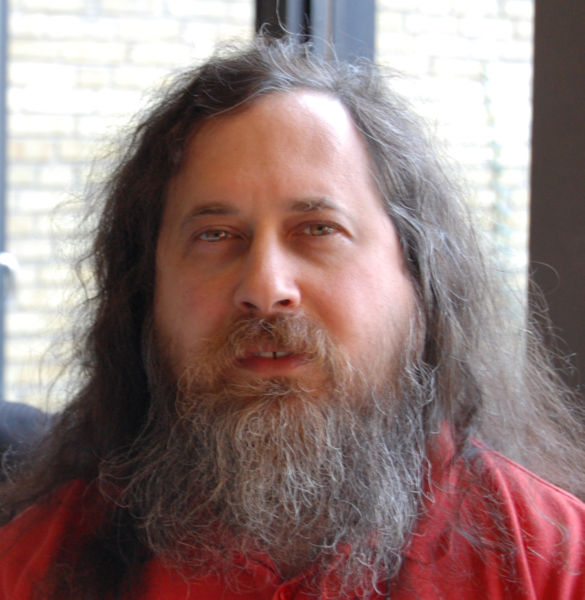
\includegraphics{img/richard}
			\end{column}
			\end{columns}
			
		\end{frame}
		
	\subsection{GNU}
		\begin{frame}
		 	\frametitle{GNU Projesi ve GPL}
			\begin{columns}
			\begin{column}[l]{5cm}
				\begin{itemize}[<+->]
					\item UNIX Modeli
					\item GNU's NOT UNIX
					\item İşletim Sisteminin Çekirdek (Kernel) Dışındaki Parçaları
					\item GPL(Genel Kamu Lisansı) 1991
					\item Linux Çekirdeği ve Bütünleşme
				\end{itemize}
			\end{column}
			\begin{column}[r]{5cm}		
				
\includegraphics{img/gnukucuk.jpg}
			\end{column}
			\end{columns}


		\end{frame}
	\subsection{GPL}
		\begin{frame}
		 	\frametitle{GPL (General Public Licence)}
			Açık Kaynak kodlu ve Özgür!
			\begin{itemize}
			 \item Programı her türlü ihtiyaç için çalıştırma
			 \item İhtiyaçlarına göre kodlarını değiştirebilme (Örnek: Amarok, blobby)
			 \item Arkadaşlarınızla paylaşabilme
			 \item Değiştirdiğiniz halini tekrar paylaşabilme ve hatta satabilme
			\end{itemize}

		\end{frame}


	\subsection{Açık Kaynak (Open Source)}
		\begin{frame}
		 	\frametitle{Açık Kaynak Kodlu Yazılım}
			\begin{itemize}
			 \item Özgür Yazılımdan Farklı
			 \item Kodlar Açık
			 \item Dağıtma izni olmayabilir
			 \item Kaynağın açık olması güvenilirliği arttırır
			 \item Microsoft Açık Kaynak iş modelinden şikayetçi ama mecburen açık kaynağa yöneliyor.
			\end{itemize}
		\end{frame}
	\subsection{Yönetici Aranıyor}
		\begin{frame}
		 	\frametitle{GNU hazır, peki ya Linux?}
				\begin{itemize}
				\item Programlar hazır
				\item Yönetecek çekirdek yok!
				\item Linus devreye giriyor
				\end{itemize}
		\end{frame}
		\begin{frame}
		 	\frametitle{Linus Torvalds}
				\begin{center}
					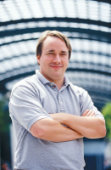
\includegraphics{img/linus.jpg}
				\end{center}
		\end{frame}
		



\section{Ne?}
	\subsection{İşletim Sistemi (Operating System)}
%		\includegraphics{img/trafikcanavari.jpg}
		\begin{frame}
			\frametitle{İşletim Sistemi Nedir?}
			\begin{itemize}
			 \item Patron
			 \item Trafik Polisi 
			 \item Çevirmen
			 \item Muhatabınız 
			 %Sizin bilgisayar sandığınız şey. Aslında yok öyle iki tıkla program açmak
			\end{itemize}

		\end{frame}

	\subsection{Çekirdek}
		\begin{frame}
		 	\frametitle{Çekirdek Nedir? Yenir mi?}
			\begin{itemize}
			 \item Aslında Linux=Çekirdek
			 \item Sürücüleri (Driver)  içerir
			 \item Modüler bir yapıdadır
			 \item Donanım Yönetimi (Bellek, İşlemci, Görüntü, Ağ, ...)
			 \item Donanım - Yazılım İletişimi			 
			 \item Linux 3.13
			 \item Her yerde kullanılıyor: PC'ler, Google Android, Cep Telefonları, PDA'ler, Casio Hesap Makineleri, Uzay Mekikleri, Robotlar
			 

			\end{itemize}
			
		\end{frame}

	\subsection{GNU/Linux}
		\begin{frame}
		\begin{center}
 		 
\includegraphics{img/linux.png}
		\end{center}
		\end{frame}

		\begin{frame}
			\frametitle{Linux Nasıl Ortaya Çıktı?}
			%\begin{columns}
			 %\begin{column}[l]{7cm}
				\begin{itemize}
					\item Linus Torvalds ve Yetersiz Minix
					\item Yeni bir çekirdek
					\item Linus + UNIX = Linux
					\item Laynıks, Lünüks değil; Linuks
				\end{itemize}  
			 %\end{column}
			%\begin{column}[r]{5cm}
			 %\includegraphics*[0in,0in][10in,10in]{linus.jpg}
			%\end{column}

			%\end{columns}


		\end{frame}
	
	\subsection{Dağıtım (Distribution)}
		\begin{frame}
		 	\frametitle{Dağıtım Nedir? Neleri içerir?}
			Dağıtım = Çekirdek ve Uygulamalar paketi.\\ Uygulamalar ihtiyaca göre seçilir. Dağıtımlar şu araçları içerir:\\
			\begin{itemize}
			 \item Kurulum Aracı (Installer)
			 \item Çekirdek (Kernel)
			 \item Uygulamalar (Applications)
			 \item Yapılandırma Araçları (Configuration Tools)
			 \item Paket Yöneticisi (Package Manager)
			\end{itemize}

		\end{frame}
		
		\begin{frame}
		 	\frametitle{Dağıtımlar}
			\begin{itemize}
			 \item Ubuntu/Kubuntu/Xubuntu
			 \item Mint			 
			 \item Arch
 			 \item Fedora
			 \item Pardus
			 \item SuSE
			 \item RedHat
			 \item Debian
			\end{itemize}
		\end{frame}


	\subsection{Masaüstü Ortamı (Desktop Environment)}
		\begin{frame}
		 	\frametitle{Masaüstü Ortamları}
				\begin{itemize}
				 \item KDE
				 \item Unity (Ubuntu Kullanıyor)
				 \item Gnome
				 \item Cinnamon (Mint Kullanıyor)
				 \item Xfce (Xubuntu kullanıyor)
				 \item Enlightenment
				\end{itemize}

		\end{frame}
 

\section{Neden?}
	\subsection{Neden Linux?}
		\begin{frame}
		 	\frametitle{Sebep?}
			\begin{itemize}[<+->]
			 \item Virüslerden korunmak için (format yok!)
			 \item Sistem istikrarı ve başarım için (defrag yok! donma yok!)
			 \item Tasarruf için (lisans ücreti yok!)
			 \item Sistemle beraber her şeyin(program ve sürücüler!) hazır gelmesi için (ek kurulum yok!)
			 \item Tüm yazılımlarınızı birkaç tıkla güncelleyebilmeniz için
			 \item Korsan yazılım kullanmamak için
			 \item Program aramaktan bıkmamak için
			 \item Düşük donanımla yüksek kalite masaüstleri için (para vermek yok!)
			 \item Özgürlük için (beklemek yok!)
			 \item Mutlu olmak için
			 \item Yan etkisi: araştırmacı ruhun ortaya çıkması
			\end{itemize}

		\end{frame}

		\begin{frame}
		 \begin{center}
			 
\includegraphics{img/bgl.png}
		\end{center}
		
		\end{frame}

	%\subsection{Neden Mac?}
	\subsection{Neden Windows?}
		\begin{frame}
		 	\frametitle{Niye ki?}
			\begin{itemize}[<+->]
			 \item İflah olmaz bir oyun hastasısınız (Steam)
			 \item Bazı programların Linux karşılığı yok (Wine)
			 \item Donanımınız Linuxla anlaşamadı (Hata raporu)
			 \item Yedekte dursun diye (Hepimiz insanız)
			 \item Microsoft'a hayransınız (E, olabilir...)
			 \item Para harcamaktan hoşlanıyorsunuz (Yok artık!)
			\end{itemize}

		\end{frame}
	
	\subsection {Linux'un Eksileri}
		\begin{frame}
			\frametitle{Nesi eksik ki?}
			\begin{itemize}[<+->]
			 \item Donanım Uyuşmazlığı (Üstesinden gelinebilir)
			 \item Paket standardının olmaması (Virüslere engel)
			 \item Bazı programların Linux sürümünün olmaması (Kullanıcı az)
			\end{itemize}

		\end{frame}



\section{Kim?}
	\subsection{Türkiye'de}
		\begin{frame}
		 
			\frametitle{Türkiye'de Kim Kullanıyor?}
			\begin{columns}
			\begin{column}[l]{5cm}
				\begin{itemize}
					\item MİT
					\item Türk Silahlı Kuvvetleri
					\item Başbakanlık
					\item TCMB
					\item TÜBİTAK
					\item Tepe İnşaat
					\item Show TV
				\end{itemize}
			\end{column}
			\begin{column}[r]{5cm}
				\begin{itemize}
					\item Finansbank
					\item HSBC
					\item Citibank
					\item Ziraat Bankası
					\item ODTÜ
					\item İTÜ
					\item ÇOMÜ
					\item Bilgi Üniversitesi
				\end{itemize}
			\end{column}
			\end{columns}

		\end{frame}

	\subsection{Dünya'da}
		\begin{frame}
		 	\frametitle{Linux'u Dünya'da Kim Kullanıyor?}
			\begin{columns}
			\begin{column}[l]{5cm}
				\begin{itemize}
					\item NASA
					\item Google
					\item IBM
					\item Yahoo
					\item HP
					\item Oracle
				\end{itemize}
			\end{column}
			\begin{column}[r]{5cm}
				\begin{itemize}
					\item Nokia
					\item Sony Ericsson
					\item Siemens
					\item Samsung
					\item Boeing
					\item General Motors
					\item Hyundai	
				\end{itemize}
			\end{column}
			\end{columns}

		\end{frame}
\part{Hadi Bakalım}
\section {Hadi Bakalım}
	
	\subsection{Nasıl Deneyeceğim?}
	\begin{frame}
		\frametitle{İşte Böyle}
			Alışkanlıklarınızın esiri olmayın!
			\begin{itemize}[<+->]
			\item Çalışan(Live) CD'ler, USB diskler
			\item Vmware / Virtual Box (Virtualization)
			\item WUBI - Windows üzerinde exe çalıştırarak
			\item Gerçek Kurulum
			\begin{itemize}
 				\item Tüm diske
				\item Windows'un yanına ayrı bir bölüme (partition)
				\item Harici bir diske
				\item USB Flash Diske (4GB)
			\end{itemize}

			%Pardus'un sitesinden
			\end{itemize}
	\end{frame}

	\subsection {Yardım?}
	\begin{frame}
		\frametitle{Nasıl yardım alacağım?}
		\begin{itemize}[<+->]
		 \item \color{brown}Google
		 \item IRC Sohbet Kanalı - irc.freenode.org \#pardus
		 \item \color{black}Linux Kullanıcıları Listesi - http://liste.linux.org.tr
		 \item Ubuntu/Mint Forumları
		 \item Diğer Forumlar
		 \item Kurumsal Destek: Özgür Yazılım A.Ş.
			 
		\end{itemize}

	\end{frame}
	
	\subsection{Siz sormadan...}
	\begin{frame}
	 	\frametitle{Siz sormadan cevaplayayım}
		\begin{itemize}[<+->]
			\item Linux ile her şeyi yapabilir miyim?
			\item Linux gerçekten hiç çökmüyor mu?
			\item Linux bu kadar iyi ise neden herkes Windows kullanıyor?
			\item Linux, Microsoft'a bir tepki mi?
			\item Microsoft'ta teknik desteği kurumdan alabiliyorum, Linux'ta üst merci olarak nereye başvuracağım?
			\item Neden tek bir Linux dağıtımı yok? (Değiştirme özgürlüğü)
			\item Linux ne zaman paralı olacak?
			\item Deli mi bu özgür yazılımcılar? Aç kalmıyorlar mı? (follars.com)
		\end{itemize}

	\end{frame}
	
% --------------------PARDUS----------------------------------
	\subsection{Şimdi ne olacak?}


	\begin{frame}
	 	\frametitle{Mint ya da Ubuntu}
		\begin{itemize}[<+->]
		 \item Bu iki dağıtımdan birini kurarak başlayabilirsiniz.
		 \item Okulda özgür yazılım topluluğu kurabilir, Linux dünyasına girerken birbirinize destek olabilirsiniz.
		 \item Özgür Yazılım Günleri ve Özgür Web Günleri konferanslarına katılarak kendinizi geliştirebilir, yeni şeyler öğrenebilirsiniz.
		 \item Linux'a başladığınıza göre Python, Ruby, Go gibi yeni nesil dillerle birlikte Java'yı bile konsol sayesinde daha etkin kullanabilirsiniz.
		\end{itemize}

	\end{frame}

% -------------------------------------------------------------
	\subsection{Duyurular}
	\begin{frame}
	\frametitle{Özgür Yazılım Günleri}
			Bahçeşehir Üniversitesi, 28-29 Mart
			\begin{itemize}
				\item http://www.ozguryazilimgunleri.org.tr/
			\end{itemize}
	\end{frame}

	\subsection{Sorularınız?}
	\begin{frame}
	 	\frametitle{Sorularınız...}
		\begin{center}
		 ?
		\end{center}
		
	\end{frame}


\end{document}
    